\documentclass[10pt]{article}
\usepackage[utf8]{inputenc}
\usepackage[a4paper,height=24cm,width=13cm]{geometry}
\usepackage[italian]{babel}
\usepackage{amssymb}
\usepackage{dsfont}
\usepackage{calc}
\usepackage{graphicx}
\usepackage{pstricks}
\usepackage{pst-node}
\usepackage{fourier}
\usepackage{euscript}
\usepackage{amsmath,amssymb, amsthm}

\def\lh{\textrm{lh}}
\def\phi{\varphi}
\def\P{\EuScript P}
\def\M{\EuScript M}
\def\D{\EuScript D}
\def\U{\EuScript U}
\def\S{\EuScript S}
\def\sm{\smallsetminus}
\def\niff{\nleftrightarrow}
\def\ZZ{\mathds Z}
\def\NN{\mathds N}
\def\PP{\mathds P}
\def\QQ{\mathds Q}
\def\RR{\mathds R}
\def\<{\langle}
\def\>{\rangle}
\def\E{\exists}
\def\A{\forall}
\def\0{\varnothing}
\def\imp{\rightarrow}
\def\iff{\leftrightarrow}
\def\IMP{\Rightarrow}
\def\IFF{\Leftrightarrow}
\def\range{\textrm{im}}
\def\Mod{\textrm{Mod}}
\def\Aut{\textrm{Aut}}
\def\Th{\textrm{Th}}
\def\acl{\textrm{acl}}
\def\eq{{\rm eq}}
\def\tp{\textrm{tp}}
\def\equivL{\stackrel{\smash{\scalebox{.5}{\rm L}}}{\equiv}}
\def\swedge{\mathbin{\raisebox{.2ex}{\tiny$\mathbin\wedge$}}}
\def\svee{\mathbin{\raisebox{.2ex}{\tiny$\mathbin\vee$}}}

\newcommand{\labella}[1]{{\sf\footnotesize #1}\hfill}
\renewenvironment{itemize}
  {\begin{list}{$\triangleright$}{%
   \setlength{\parskip}{0mm}
   \setlength{\topsep}{0mm}
   \setlength{\rightmargin}{0mm}
   \setlength{\listparindent}{0mm}
   \setlength{\itemindent}{0mm}
   \setlength{\labelwidth}{3ex}
   \setlength{\itemsep}{0mm}
   \setlength{\parsep}{0mm}
   \setlength{\partopsep}{0mm}
   \setlength{\labelsep}{1ex}
   \setlength{\leftmargin}{\labelwidth+\labelsep}
   \let\makelabel\labella}}{%
   \end{list}}
%\def\ssf#1{\textsf{\small #1}}
\newcounter{ex}
\newenvironment{exercise}{\clearpage\addtocounter{ex}{1}\textbf{Esercizio \theex.\quad}}{}
\newcounter{sol}
\newenvironment{solution}{\addtocounter{sol}{1}\textbf{Soluzione \theex.\quad}}{}
\pagestyle{empty}
\parindent0ex
\parskip2ex
\raggedbottom
\def\nsR{{}^*\kern-.2ex\RR}
\def\nsN{{}^*\kern-.2ex\NN}
\def\nsQ{{}^*\kern-.2ex\QQ}
\def\ns{{}^*\kern-.2ex}
\def\st{{\rm st}}
\def\ssf#1{\textsf{#1}}
\renewcommand{\baselinestretch}{1.3}


\usepackage{fancyhdr}
\pagestyle{fancy}
\lfoot{Teoria dei Modelli a.a.~2020/21}
\rhead{}
\rfoot{\rput(1.5,-0.5){\small\thepage}}
\cfoot{}

%
% INDICARE NOME E COGNOME DI TUTTI GLI AUTORI
%
\lhead{Gabriele Rastello}
%
\begin{document}
   
\begin{exercise}
  Let $L = \{<\}$ and let $N$ be a $\omega_1$-saturated extension of $\QQ$. 
  Prove that there is an embedding $f:\RR \to  N$. Is it elementary? Can it be an isomorphism?
\end{exercise}

\begin{solution}
  From Theorem 9.6 \(N\) \(\omega_1\)-saturated implies that \(N\) is \(\omega_1\)-rich in the category \(\M\) with elementary maps as arrows.
  As \(N\) is an extension of \(\mathbb{Q}\) there is an elementary embedding \(\mathbb{Q}\hookrightarrow N\); this can be regarded as an elementary map \(\mathbb{R}\to N\) of cardinality \(<\omega_1\).
  Now using that \(N\) is \(\omega_1\) rich together with the finite character of morphisms (c2 from Definition 7.1) we can extend that map to obtain an embedding \(f\)
  of \(\mathbb{R}\) in \(N\) that is elementary.

  Finally suppose that \(f\) is an isomorphism and consider the type \(p(x) = \big\{n < x\colon n\in\mathbb{N}\big\}\) with parameters in \(\mathbb{N}\) of cardinality \(<\omega_1\).
  This type is realized in \(N\) by \(\omega_1\)-saturation.
  Now, since \(f\) is an isomorphism, there must be a \(x^*\in\mathbb{R}\) that realizes the type in \(\mathbb{R}\) but this is absurd.
\end{solution}

\begin{exercise}
  Let $M$ and $N$ be elementarily homogeneous structures of the same cardinality $\lambda$. Suppose that $M\models\E x\, p(x)\,\IFF\,N\models\E x\, p(x)$ for every $p(x)\subseteq L$ such that $|x|<\lambda$. Prove that the two structures are isomorphic. (Hint: see Theorem 7.8)
\end{exercise}

\begin{solution}
  We would like to do a back-and-forth construction but in order to do so we need a ``morphism extension lemma''.

  Let \(k\colon M\to N\) be an elementary map such that \(|\textrm{dom}(k)|<\lambda\).
  Now pick \(b\in N\) (that we can assume to be outside \(\textrm{im}(k)\)) and consider the type
  \[p(x) = \text{tp}_N\big(\textrm{im}k, b\big)\]
  where we consider \(\textrm{im}(k)\) as a tuple.
  Since \(|\textrm{im}(k)|<\lambda\) by assumption \(p(x)\) is realized by some \(a\in M^{|\textrm{im}(k)|}\) and \(c\in M\).
  Now let \(j\colon N\to M\) be the map with \(\textrm{dom}(j) = \textrm{im}(k) \cup \{b\}\) that sends the tuple \(\textrm{im}(k)\) to the tuple \(a\) and the element \(b\) to the element \(c\).
  This map is elementary because given \(\varphi(x)\in L\) and \(a\in N^{|x|}\) such that \(N\models\varphi(a)\) we have \(\varphi(x)\in p(x)\) and thus \(M\models \varphi(ja)\).
  The composition of elementary maps is elementary so \(j\circ k\colon M\to M\) is elementary and, by \(\lambda\)-homogeneity, extends to an automorphism \(h\colon M\to M\).

  Now consider the map \(k'\colon M\to N\) with \(\textrm{dom}(k') = \textrm{dom}(k)\cup \big\{h^{-1}c\big\}\) defined as \(k' = j^{-1}\circ h\).
  This is an elmentary map and an extension of \(k\) such that \(b\in \textrm{im}(k')\).
  \begin{figure}[h]
    \begin{center}
      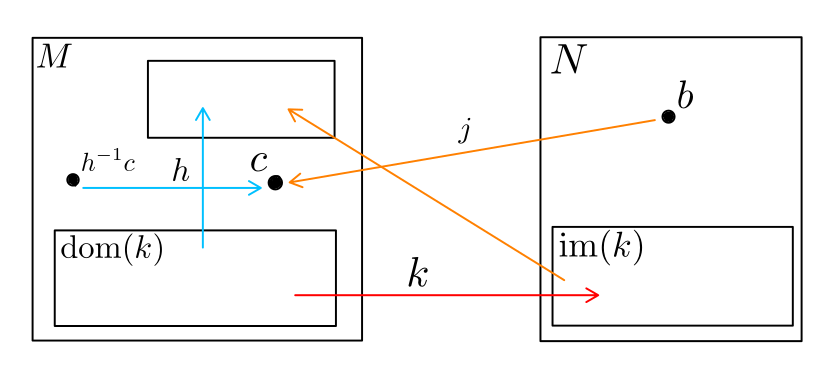
\includegraphics[width=0.75\textwidth]{fig1.png}
    \end{center}
  \end{figure}
  
  We can now obtain an isomorphism by a back-and-forth construction using the above ``morphism extension lemma'' and familiar induction techniques.
\end{solution}

\begin{exercise}
  Let $A\subseteq N\models T_{\rm acf}$ what is the cardinality of $S_x(A)$, where $|x|=1$? Recall that $S_x(A)$ is the set of complete types $p(x)\subseteq L(A)$, finitely consistent in $N$.

  Answer the same question for $A\subseteq N\models T_{\rm rg}$.
\end{exercise}

\begin{solution}

  \textbf{Algebraically closed fields.}
  Consider \(\overline{A}\) made of all \(a\in\U\) (with \(\U\) some monster model) such that there is a polinomial equation \(\varphi_a(x)\in L(A)\) for which \(\varphi_a(a)\) is true.
  Since \(T_{\rm acf}\) has quantifier elimination we can assume all formulas to be polynomial (un)equations eventually combined with connectives.

  Consider \(p(x)\in S_x(A)\) and let \(a\) be a realization of \(p\).
  By completeness unless \(p\) is the type of all polynomial unequations there is some polynomial equation \(\varphi_a(x)\in p\) such that \(\varphi_a(a)\) is true and so \(a\in\overline{A}\).
  Now if \(b\in\overline{A}\) is another realization of \(p\) then \(\varphi_a(b)\) must be true as well and so \(p\) has a finite number of realizations (or \(\varphi_a(x)\) would have arbitrarily large degree).
  As we only ignored one type \(|S_x(A)| \leq |\overline{A}|\).

  Now consider \(a\in\overline{A}\) and let \(p(x)\in S_x(A)\) be the unique (by completeness) type with realization \(a\).
  By remembering that \(p(x)\) has only a finite number of realizations we have \(|\overline{A}| \leq |S_x(A)|\).
  So, in the end, \(|S_x(A)| = |\overline{A}|\).

  Finally if \(A\) is infinite then \(|A| = |\overline{A}|\) and if \(A\) is finite then \(|\overline{A}|=\aleph_0\).

  \textbf{Random graphs.}
  We know that \(T_{\rm rg}\) has quantifier elimination so we can assume that all formulas in our types are of the kind \(r(x, a)\) or \(\neg r(x,a)\) for some \(a\in A\), eventually combined with the binary connectives.

  By completeness every type \(p(x)\in S_x(A)\) is completely determined by a binary choice for every \(a\in A\) and thus \(S_x(A)\) is in bijection with the set \(2^A\).
  So we conclude \(|S_x(A)| = |2^A|\).
\end{solution}
\end{document}

